%%%%%%%%%%%%%%%%%%%%%%%%%%%%%%%%%%%%%%%%%%%%%%%%%%%%%%%%%%%%%%%
%
% Time representation
%
%%%%%%%%%%%%%%%%%%%%%%%%%%%%%%%%%%%%%%%%%%%%%%%%%%%%%%%%%%%%%%%%

This section is devoted to specify the representation of time within the framework of the possibility theory. First of all, the specification for a single ill-known temporal point will be explained. Then, the formal specification and the related constraints are given for an ill-known valid-time interval.

\subsection{\label{subsec:ill-known-point-rep}Ill-known time point}
An ill-known time point $X$ is a precise time point that, for some reason, is not fully specified. Note that $X$ has only one possible value but that value is unspecified.

\begin{definition}
\label{def:ill-known-time-point}
\textbf{Ill-known time point.}\\
Consider a time domain $\T$; the uncertainty about the values of the ill-known time point $X$ is given by the possibility distribution $\pi_X$:
\begin{equation}
\label{eq:ill-known-time-point}
\Pi(X) = \pi_X(t) \in \left[0,1\right] , t \in \T
\end{equation}
\end{definition}

It is also possible to specify an ill-known time point by a convex combination of ill-known constraints, as shown by equation \eqref{eq:ill-known-value-def-by-const-unc}.



\begin{definition}
\label{def:ill-known-domain}
\textbf{Domain for an ill-known time point.}\\
Consider $\Pow(\T)$ the set of all the possibility distributions over $\T$, and the three fuzzy constants \emph{UNKNOWN} $=\left\lbrace 1/t, \forall t \in \T \right\rbrace$, \emph{UNDEFINED} $=\left\lbrace 0/t,\forall t \in \T \right\rbrace$ and \emph{NULL} $=\lbrace 1/$ \emph{UNKNOWN}, $1/$ \emph{UNDEFINED} $\rbrace$. The domain for an ill-known time point $X$ is given by: 
\begin{align}
\label{eq:ill-known-domain}
\Dom (X) =  \lbrace \Pow(\T) & \cup \mbox{\emph{UNKNOWN}} \\
\nonumber
&\cup \mbox{\emph{UNDEFINED}} \\
\nonumber
&\cup \mbox{\emph{NULL}} \rbrace
%
\end{align}
\end{definition}




\subsubsection{\label{subsubsec:ill-known-time-datatypes}Datatypes}
The data type for the representation of an ill-known time point allows the representation of the values shown in Table \ref{tbl:time-point-types}
%The datatypes for an  $X$ are shown in Table \ref{}.
\begin{samepage}
\vglue13pt
%\begin{table}[htbp]
\tcap{\label{tbl:time-point-types}Values for the time point data type.}
\centerline{\small DIFFERENT VALUES FOR A TIME POINT}
\vglue-6pt
\centerline{\small\baselineskip=13pt
\begin{tabular}{c p{0.4\columnwidth} p{0.3\columnwidth}}\\
Subtype & Value & Representation \\
\hline
1 & A single time point &  $1/x, x \in \T$\\
2 & A possibility distribution in the numeric domain & A fuzzy number or a fuzzy interval.\\
3 & An unknown value & \textbf{UNKNOWN}$= \lbrace1/t,\forall t \in \T \rbrace$\\
4 & An undefined value & \textbf{UNDEFINED}$= \lbrace 0/t,\forall t \in \T \rbrace$\\
5 & A null value & \textbf{NULL} $=\lbrace 1/$Unknown, 1/Undefined $\rbrace$\\
\hline\\
\end{tabular}
}
\end{samepage}

%Example of different uses of the ill-known time value.
\begin{example}
Consider a historical database with data from medieval diplomatic documents. The following fields are stored: the digital identifier \emph{ID} which is the primary key  and the estimated time when the document was sent (field \emph{Date}). Table \ref{tbl:sample-time-point} contains some example data from this database. 
\end{example}

\vglue13pt
%\begin{table}[htbp]
\tcap{Sample of the historical database}
%\centerline{\small DATA TYPES}
\vglue-6pt
\centerline{\small\baselineskip=13pt
\begin{tabular}{c c}\\
\textbf{ID} & Date\\
\hline
23454 & Unknown \\ 
34563 & 11/12/1204 \\
12211 & $\left[7/2/1204,30,30\right]$ \\
23455 & $\left[10,10/6/1204,20/6/1204,15 \right]$ \\
\hline\\
\end{tabular}
\label{tbl:sample-time-point}
} 
 
In that database, for the document with ID=23454, all the dates in the domain are equally possible. Nevertheless, the document 34563 was sent in the crisp (exact) date 11/12/1204. The time for documents 12211 and 23455 are specified with several possibility distributions. The first one is also known as a fuzzy number whereas the second one is also known as a fuzzy interval, as explained in Section \ref{sec:prelim}.
 
%\end{example}
 
 


\subsection{\label{subsec:ill-known-interval}Ill-known time interval}



An ill-known time interval denoted by $\left[X, Y\right]$ is a precise time interval whose boundaries are not precisely known. %The ill-known time interval is defined by two ill-known  time points, namely $X$,$Y$. The evaluation of the ill-known time interval is given by equations \eqref{ill-known-pos},\eqref{ill-known-nec}.

\begin{definition}
\emph{Ill-known time interval}
Let $\T$ be the time domain, and $X$, $Y$ two ill-known values in the time domain. An ill-known time interval is given by $\left[X, Y\right]$. The evaluation of the ill-known time interval is given by equations \eqref{ill-known-pos},\eqref{ill-known-nec}. We will note $\I_{PVP}$ the set of all the ill-known time intervals.

\end{definition}


% In order to know whether all the points in the crisp time interval $I=\left[a, b\right]$ are within the boundaries of the ill-known time interval $\left[X, Y\right]$ we define the following two ill-known constraints $C_{1}, C_{2}$ 
% \begin{eqnarray}
% \label{eq:constraint-c1}
% C_1\stackrel{\triangle}{=}\left(\geq,X\right)  \\
% \label{eq:constraint-c2}
% C_2\stackrel{\triangle}{=}\left(\leq,Y\right)
% \end{eqnarray}
% Note that the boolean operator applied to the constraints is $\bool=\wedge$. Hence, the construct of both constraints is $C_1 \wedge C_2$
% This means that we want to know if all the points in the interval $I$ are greater than or equal to $X$ and, at the same time, smaller than or equal to $Y$.
% %\end{definition}
% 
% %% equations for the poss and nec!!
% The simplified equations for the possibility and the necessity measures are~\cite{Pons2011}:
% \begin{eqnarray}
% \label{eq:time-interval-pos}
% \Pos\left(\lambda([a,b])\right)&=&\\
% \nonumber
% \min\bigg(\sup_{a\leq w}\pi_{X}(w),\sup_{b\geq w}\pi_{Y}(w)\bigg)\\
% \label{eq:time-interval-nec}
% \Nec\left(\lambda([a,b])\right)&=&\\
% \nonumber
% \min\bigg(\inf_{a>w}1-\pi_{X}(w),\inf_{b<w}1-\pi_{Y}(w)\bigg).
% \end{eqnarray}




\subsubsection{\label{subsubsec:open-interval}Open ill-known time intervals}
Quite often, the user may want to specify time intervals with open boundaries in one or both endpoints. Consider an ill-known time interval $\left[X, Y\right]$. Then it is possible to distinguish between the following two types of open intervals:
%\begin{enumerate}
%\item
\begin{definition}
\textbf{Completely unknown time interval}: Both starting and ending points are unknown, therefore the whole interval is unknown.
%specified by the \emph{UNKNOWN} constant. Due to the representation, both endpoints, say $X$ and $Y$, are stored. Thus, the interval is stored as $[$ \emph{UNKNOWN}, \emph{UNKNOWN} $]$. 
\end{definition}

%\item
\begin{definition}
\textbf{Semi-open time interval}: Only one of the two ill-known endpoints for the time interval $\left[X, Y\right]$ is unknown. Example \ref{ex:open-time-interval} and Figure \ref{fig:example-open-time-interval} illustrates a left open time interval.
% Note that due to the ill-known constraints $C_{1}, C_{2}$ it is not possible a representation like $[$ \emph{UNKNOWN} $, Y]$ or $[X, $ \emph{UNKNOWN} $]$. The solution adopted for this problem is explained in the following paragraph. 
\end{definition}
%\end{enumerate}

\subsubsection{\label{subsubsec:representation-semi-open}Representation of semi-open time intervals}
As mentioned before, the problem resides in the representation of this kind of interval. 

% In order to get a short representation for these intervals, two constants are defined: $FB$ -\emph{From the Beginning}- it is only valid for the left value of the interval and $UC$ -\emph{Until Changed}- (this name is usual in the temporal database community, see ~\cite{Jensen1994}) which is only valid for the right value of the interval. Note that these two constants are aliases for a function that obtains both possibility and necessity measures. 

Because of the ill-known constraints $C_{1}, C_{2}$, a function called \emph{Open} should be defined in order to deal with a proper representation of these intervals.

\begin{definition}
\label{def:open-func}
$Open(C)$\\
Consider an ill-known value $T$, a binary relationship $B_r \in \left \lbrace \leq, <, >, \geq\right \rbrace$ and the constraint $C\stackrel{\triangle}{=}\left(R,T\right)$.
The function $\Open(C) = \left(I_p(C), I_n(C) \right)$ provides both possibility and necessity measures for all the points in the open part of a semi-open ill-known time interval.

The possibility and necessity measures are defined by:
\begin{eqnarray}
\label{eq:open-pos-nec}
I_p \left(C \right) &=& \Big(\sup_{r\in\T, r \Rp\  w}\pi_{T}(w)\Big)\\
I_n \left(C \right) &=& \Big(\inf_{r\in\T, r \Rn\  w}1-\pi_{T}(w)\Big)
\end{eqnarray}
Where the values for the binary relations $\Rp$ and $\Rn$ are shown in Table \ref{tbl:open-pos-nec-rels}.
\end{definition} 

\begin{samepage}
\vglue13pt
%\begin{table}[htbp]
\tcap{Relations for the $\Open(C)$ function. Depending on the relation $B_r \in \left \lbrace \leq, <, >, \geq\right \rbrace$ in the constraint $C$, the values for $\Rp$ and $\Rn$ are shown.}
\centerline{\small Relations}
\vglue-6pt
\centerline{\small\baselineskip=13pt
\begin{tabular}{c c c}\\
\hline
Constraint & $\Rp$ & $\Rn$\\ \hline
$C\stackrel{\triangle}{=}\left(<,T\right)$ & $>$ & $\leq$ \\
$C\stackrel{\triangle}{=}\left(\leq,T\right)$ & $\geq$ & $<$ \\
$C\stackrel{\triangle}{=}\left(>,T\right)$ & $<$ & $\geq$ \\
$C\stackrel{\triangle}{=}\left(\geq,T\right)$ & $\leq$ & $>$ \\
\hline\\
\end{tabular}
\label{tbl:open-pos-nec-rels}
}
\end{samepage}

As explained before, the constants $\FB$ and $\UC$ are aliases for the function $\Open$ with the following parameters:
\begin{eqnarray}
\FB &=& \Open(C_2)\\
\UC &=& \Open(C_1)
\end{eqnarray}

Where the constraints $C_1$ and $C_2$ are given in equations \eqref{eq:constraint-c1} and \eqref{eq:constraint-c2}.

\begin{example}
\label{ex:open-time-interval}
Consider an ill-known time interval given by $\left[\FB, Y \right]$. Consider also that, in this case, $Y= \left[15/10/2012,3,4 \right] $. Figure \ref{fig:example-open-time-interval} shows the representation for $Y$. The user wants to obtain the possibility and the necessity measures for the $\FB$ part of the interval.
\end{example}

\begin{eqnarray}
\nonumber
\FB = \Open(C_2) \mbox{ with } C_2\stackrel{\triangle}{=}\left(\leq,Y\right)\\
\nonumber
I_p(C_2)= \Big(\sup_{r\in\T \geq\  w}\pi_{Y}(w)\Big)\\
\nonumber
I_n(C_2) = \Big(\inf_{r\in\T <\  w}1-\pi_{Y}(w)\Big)
\end{eqnarray}

\begin{samepage}
\vspace*{13pt}
\begin{center}
{
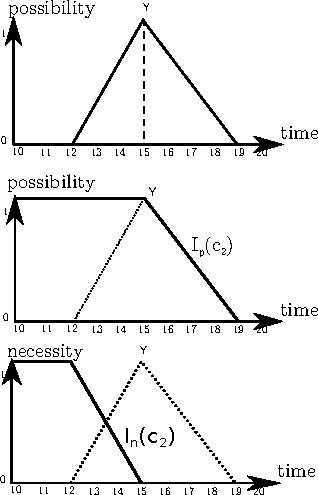
\includegraphics[scale=1]{./graphs/open-time-interval.pdf}

}
\end{center}
%\centerline{ 
\psfig{file=./graphs/Y-time-point.eps}}
\vspace*{10pt}
\fcaption{\label{fig:example-open-time-interval}Possibility distribution for $Y$, and possibility and necessity measures for the open ill-known point, $X$}
\vspace*{13pt}
\end{samepage}

% \vglue13pt
% %\begin{table}[htbp]
% \tcap{Relations for the $\Open(C)$ function.}
% \centerline{\small Relations}
% \vglue-6pt
% \centerline{\small\baselineskip=13pt
% \begin{tabular}{c c c}\\
% \hline
% $R$ & $\Rp$ & $\Rn$\\ \hline
% $<$ & $>$ & $\leq$ \\
% $\leq$ & $\geq$ & $<$ \\
% $>$ & $<$ & $\geq$ \\
% $\geq$ & $\leq$ & $>$ \\
% \hline\\
% \end{tabular}
% \label{tbl:open-pos-nec-rels}
% }



\subsubsection{\label{subsubsec:ill-known-time-interval-datatypes}Datatypes}
In order to properly represent  an ill-known time interval in a database, some datatypes are needed. Because of the ill-known constraints, not all the combinations of datatypes for each ill-known time point (see Table \ref{tbl:time-point-types}) are allowed. Table \ref{tbl:time-interval-types} shows all the possible values that can be used to represent an ill-known time interval denoted by $\left[X, Y\right]$.

\begin{samepage}
\vglue13pt
%\begin{table}[htbp]
\tcap{All the possible combination of values for the time interval $\left[X, Y\right]$. The subtypes refer to Table \ref{tbl:time-point-types}.}
\centerline{\small TIME INTERVAL DATA TYPE}
\vglue-6pt
\centerline{\small\baselineskip=13pt
\begin{tabular}{p{0.15\columnwidth} p{0.15\columnwidth} p{0.5\columnwidth}}\\
\hline
Subtype for $X$  & Subtype for $Y$  & Description\\
\hline
1 or 2 & 1 or 2 &  An ill-known time interval.\\
3 & 3 & An unknown time interval. \\
$\FB$ & 1 or 2 & A left-open time interval.\\
1 or 2 & $\UC$ & A right-open time interval.\\
\hline\\
\end{tabular}
\label{tbl:time-interval-types}
}
\end{samepage}

% Maybe an example with a database.
% \begin{example}
% 
% \end{example}


% \subsection{\label{subsec:fuzzy-allen-relations}Allen's relations}
% The Allen's relations can be represented by a Boolean combination of ill-known constraints. The constructs for the constraints are shown in Table \ref{tbl:fuzzy-allen-relations}. The possibility and necessity measures are obtained for each Boolean function as explained in Section \ref{subsec:interval-evaluation-by-ill-known-constraints} in equations \eqref{eq:conjunctive1}-\eqref{eq:negation}.
% 
% 
% \vglue13pt
% %\begin{table}[htbp]
% \tcap{\label{tbl:fuzzy-allen-relations}Constructs of constraints related to their respective Allen relations, as used in the presented work. In this table, the ill-known time interval $J = \left[X, Y\right]$ in a record $r$ has a start point described by possibilistic variable $X$ and an end point described by possibilistic variable $Y$. The crisp time interval in the user's temporal demand is denoted $I$.}
% \centerline{\small Relations}
% \vglue-6pt
% \centerline{\small\baselineskip=13pt
% \begin{tabular}{p{0.2\columnwidth} p{0.8\columnwidth} }\\
% \hline
% Allen Relation & Construct of constraints\\
% \hline
% I before J & $C_1 \triangleq \left(<,X\right)$ \\
% \hline
% I equal J & $\left(C_1 \triangleq \left(\geq,X\right)\right) \wedge \neg \left(C_2 \triangleq \left(\neq,X\right) \right) \wedge \left(C_3 \triangleq \left(\leq,Y\right) \right) \wedge \neg \left(C_4 \triangleq \left(\neq,Y\right)\right)$ \\
% \hline
% I meets J & $\left(C_1 \triangleq \left(\leq,X\right)\right) \wedge \neg \left(C_2 \triangleq \left(\neq,X\right) \right)$ \\
% \hline
% I overlaps J & $\left(C_1 \triangleq \left(<,Y\right)\right) \wedge \neg \left(C_2 \triangleq \left(\leq,X\right) \right) \wedge \neg \left(C_3 \triangleq \left(\geq,X\right) \right)$ \\
% \hline
% I during J & $\left( \left (C_1 \triangleq \left(>,X\right) \right) \wedge \left(C_2 \triangleq \left(\leq,Y\right) \right) \right) \vee \left( \left(C_3 \triangleq \left(\geq,X\right) \right) \wedge  \left(C_4 \triangleq \left(<,Y\right) \right) \right)$ \\
% \hline
% I starts J & $\left(C_1 \triangleq \left(\geq,X\right) \right) \wedge \neg \left(C_2\triangleq \left(\neq,X\right)\right)$ \\
% \hline
% I finishes J & $\left(C_1 \triangleq \left(\leq,Y\right) \right) \wedge \neg \left(C_2\triangleq \left(\neq,Y\right)\right)$ \\
% \hline\\
% \end{tabular}
% }

%\subsection{\label{subsec:time-interval-constraint}Ill-known valid time-interval}
%The representation of a possibilistic valid-time interval is given by two ill-known points: $\left[S,E \right]$ the starting and ending points respectively.  
%
%
%A valid temporal interval $\left[S,E\right]$ in the system is a combination for the values of $S$,$E$. Note that the only allowed combination of types is shown in table \ref{tbl:valid-time-interval}. 
